% Format:  Latex Orientation:  Portrait
% MASTERFILE
%
% Last change: <Thu, 2016/05/26 10:25:26 arwagner l00slwagner.desy.de>
%
\documentclass[presentation, 10pt]{beamer}
% use ``handout'' instead of ``presentation'' to create a 2 on 1 page
% handout version of the document

\mode<handout>{%
	\usepackage{pgf}
	\usepackage{pgfpages}
	\pgfpagesuselayout{2 on 1}[a4paper,border shrink=5mm]
}
\mode<presentation>{%
	\usetheme{DESY}
}
%% Setup for Beamer
\usepackage{xcolor}
\usepackage{hyperxmp}
% \usepackage[pdfa]{hyperref}
\usepackage{luatextra}
\usepackage{wasysym}
\usepackage{eurosym}
\usepackage{bookmark}
\usepackage{graphicx}
\usepackage{fontspec}
\setmainfont{Arial}
\usepackage[ngerman,english]{babel}
\usepackage{xspace}
\usepackage{tikz}

\tikzset{%
  every overlay node/.style={%
    %draw=black,fill=white,rounded corners,anchor=north west,
    draw=fzjlightblue,fill=fzjgray30,rounded corners,anchor=north west,
  },
}
% Usage:
% \tikzoverlay at (-1cm,-5cm) {content};
% or
% \tikzoverlay[text width=5cm] at (-1cm,-5cm) {content};
\def\tikzoverlay{%
   \tikz[baseline,overlay]\node[every overlay node]
}%


% General new commands an macros
\renewcommand{\emph}[1]{\structure{#1}}

\newcommand{\link}[2]{\href{#1}{~#2}}

\newcommand{\jointwo}{\textbf{JOIN$^2$}\xspace}

\newcommand{\BibTeX}{Bib\TeX}
\newcommand{\JabRef}{\link{http://jabref.sf.net}{JabRef}\xspace}
\newcommand{\Companion}[1]{\textit{\link{http://julib.fz-juelich.de/uhtbin/field-search-sort/001/PBYR/213964}{\LaTeX{} Companion}, #1}\xspace}
\newcommand{\pkg}[1]{\emph{\texttt{#1}}\xspace}

% general colour definitions
\newcommand{\smallgray}[1]{{\tiny\emph{#1}}}

\newcommand{\idR}{i.~d.~R.\xspace}
\newcommand{\va}{v.~a.\xspace}
\newcommand{\sa}{s.~a.\xspace}
\newcommand{\zB}{z.~B.\xspace}
\newcommand{\zT}{z.~T.\xspace}
\newcommand{\ggf}{ggf.\xspace}
\newcommand{\eg}{e.~g.\xspace}

\newcommand{\bs}[1]{\texttt{$\backslash$#1}}
\newcommand{\command}[2]{\texttt{\bs{#1}\{#2\}}}
% http://tex.stackexchange.com/questions/16447/beamer-top-aligning-columns-within-a-top-aligned-fram
\makeatletter
\newenvironment{topitemize}{%
   \setlength{\topsep}{0pt}
   \setlength{\partopsep}{0pt}
   \renewcommand*{\@listi}{\leftmargin\leftmargini \parsep\z@ \topsep\z@ \itemsep\z@}
   \let\@listI\@listi
   \itemize
}{\enditemize}
\makeatother


\title{DQM4HEP \\ Status and prospects}
% subtitle is required for DESY beamer, set at least a space ~
\subtitle{AIDA-2020 WP5 meeting - DESY}

\author[R. Ete]{\underline{R. Ete}, A. Pingault, T. Coates}
\institute{DESY}
\date{October 9, 2017}

\newenvironment{topitemize}{%
   \setlength{\topsep}{0pt}
   \setlength{\partopsep}{0pt}
   \renewcommand*{\@listi}{\leftmargin\leftmargini \parsep\z@ \topsep\z@ \itemsep\z@}
   \let\@listI\@listi
   \itemize
}{\enditemize}

\usepackage{makecell}
\usepackage{tikz}

%---------------------------------------------------------------------

\begin{document}

\maketitle

% %----------------------------------------------------------------------
% \begin{frame}
%   \frametitle{Summary}
%
%   \begin{itemize}
%     \item Framework presentation
%     \item Experiments running with DQM4HEP
%     \item EUDAQ / DQM4HEP interface
%     \item Current status
%     \item Ongoing and future work
%   \end{itemize}
%
% \end{frame}

% %----------------------------------------------------------------------
% \begin{frame}
%   \frametitle{Introduction}
%   \scriptsize
%   DQM systems in HEP domain :
%   \begin{itemize}
%     \item Evaluate data quality and alert users of anomalies
%     \begin{itemize}
%       \scriptsize
%       \item Are the distribution what we expect ?
%       \item Comparison between runs or old/new software version
%       \item Quick feedback from hundred of plots is challenging
%     \end{itemize}
%     \item Provide online and offline analysis
%     \begin{itemize}
%       \scriptsize
%       \item Automated data quality tests, possibly with reference histograms
%       \item Distributed system for online analysis (data collectors)
%       \item Dedicated visualization interface (Qt, Web)
%     \end{itemize}
%     \item Already developed for most of HEP experiments (i.e AMORE or CMSSW)
%   \end{itemize}
%   ~\\
%   \textbf{But ...} Based on experiment specific event format
%   \begin{itemize}
%     \item Not re-usable by other experiments
%     \item Duplicated software
%     \item Ad-hoc solution for test-beam setup monitoring
%   \end{itemize}
%   ~\\
%   Development of a generic DQM software for any HEP experiment : \textbf{DQM4HEP}
% \end{frame}



%----------------------------------------------------------------------
\begin{frame}
  \frametitle{DQM4HEP}
  \framesubtitle{Software overview}
  \footnotesize
  Key points :
  \begin{itemize}
    \item Standalone plugin system
    \begin{itemize}
      \scriptsize
      \item Plugin = C++ class in a shared library
      \item Load shared library at runtime and hook plugin class
    \end{itemize}
    \item \textbf{Generic event data model/format}. User needs to define :
    \begin{itemize}
      \scriptsize
      \item Event model
      \item Conversion Model $\leftrightarrow$ Binary
    \end{itemize}
  \end{itemize}
  ~ \\
  More general features :
  \begin{itemize}
    \item Online analysis (API)
    \item Distributed system (TCP/IP)
    \item Data collectors : event and histogram collector servers
    \item Quality test tools : interface + quality test templates
    \item Visualization interface (histograms and quality tests)
  \end{itemize}
\end{frame}


%----------------------------------------------------------------------
\begin{frame}
  \frametitle{DQM4HEP}
  \framesubtitle{Quality test API}
  \footnotesize
  \begin{block}{Monitor element}
    \begin{itemize}
      \item Wrap a ROOT TObject
      \item Optionally hold a ROOT TObject as reference
    \end{itemize}
  \end{block}
  \begin{block}{Quality test}
    \begin{itemize}
      \item Implement the logic to test a monitor element
      \item Output a quality report (quality flag, success, etc)
    \end{itemize}
  \end{block}
  One monitor element can be tested with many QTests, e.g : \\
  \begin{itemize}
    \item Kolmogorov test using a reference histogram
    \item Mean of histogram within an expected value
  \end{itemize}
  One QTest can be attached to many monitor elements, e.g :
  \begin{itemize}
    \item Test different histograms with the same gaussian distribution
  \end{itemize}
\end{frame}


%----------------------------------------------------------------------
\begin{frame}
  \frametitle{DQM4HEP}
  \framesubtitle{Online architecture}
  \begin{overlayarea}{\textwidth}{0.6\textheight}
    \begin{center}
      \includegraphics[width=0.9\linewidth]<1>{figs/GlobalArchitectureDiagramUpdated.pdf}
      \includegraphics[width=0.9\linewidth]<2>{figs/GlobalArchitectureDiagramDataFlow.pdf}
      \includegraphics[width=0.9\linewidth]<3>{figs/GlobalArchitectureDiagramUserCode.pdf}
    \end{center}
  \end{overlayarea}
  % \centering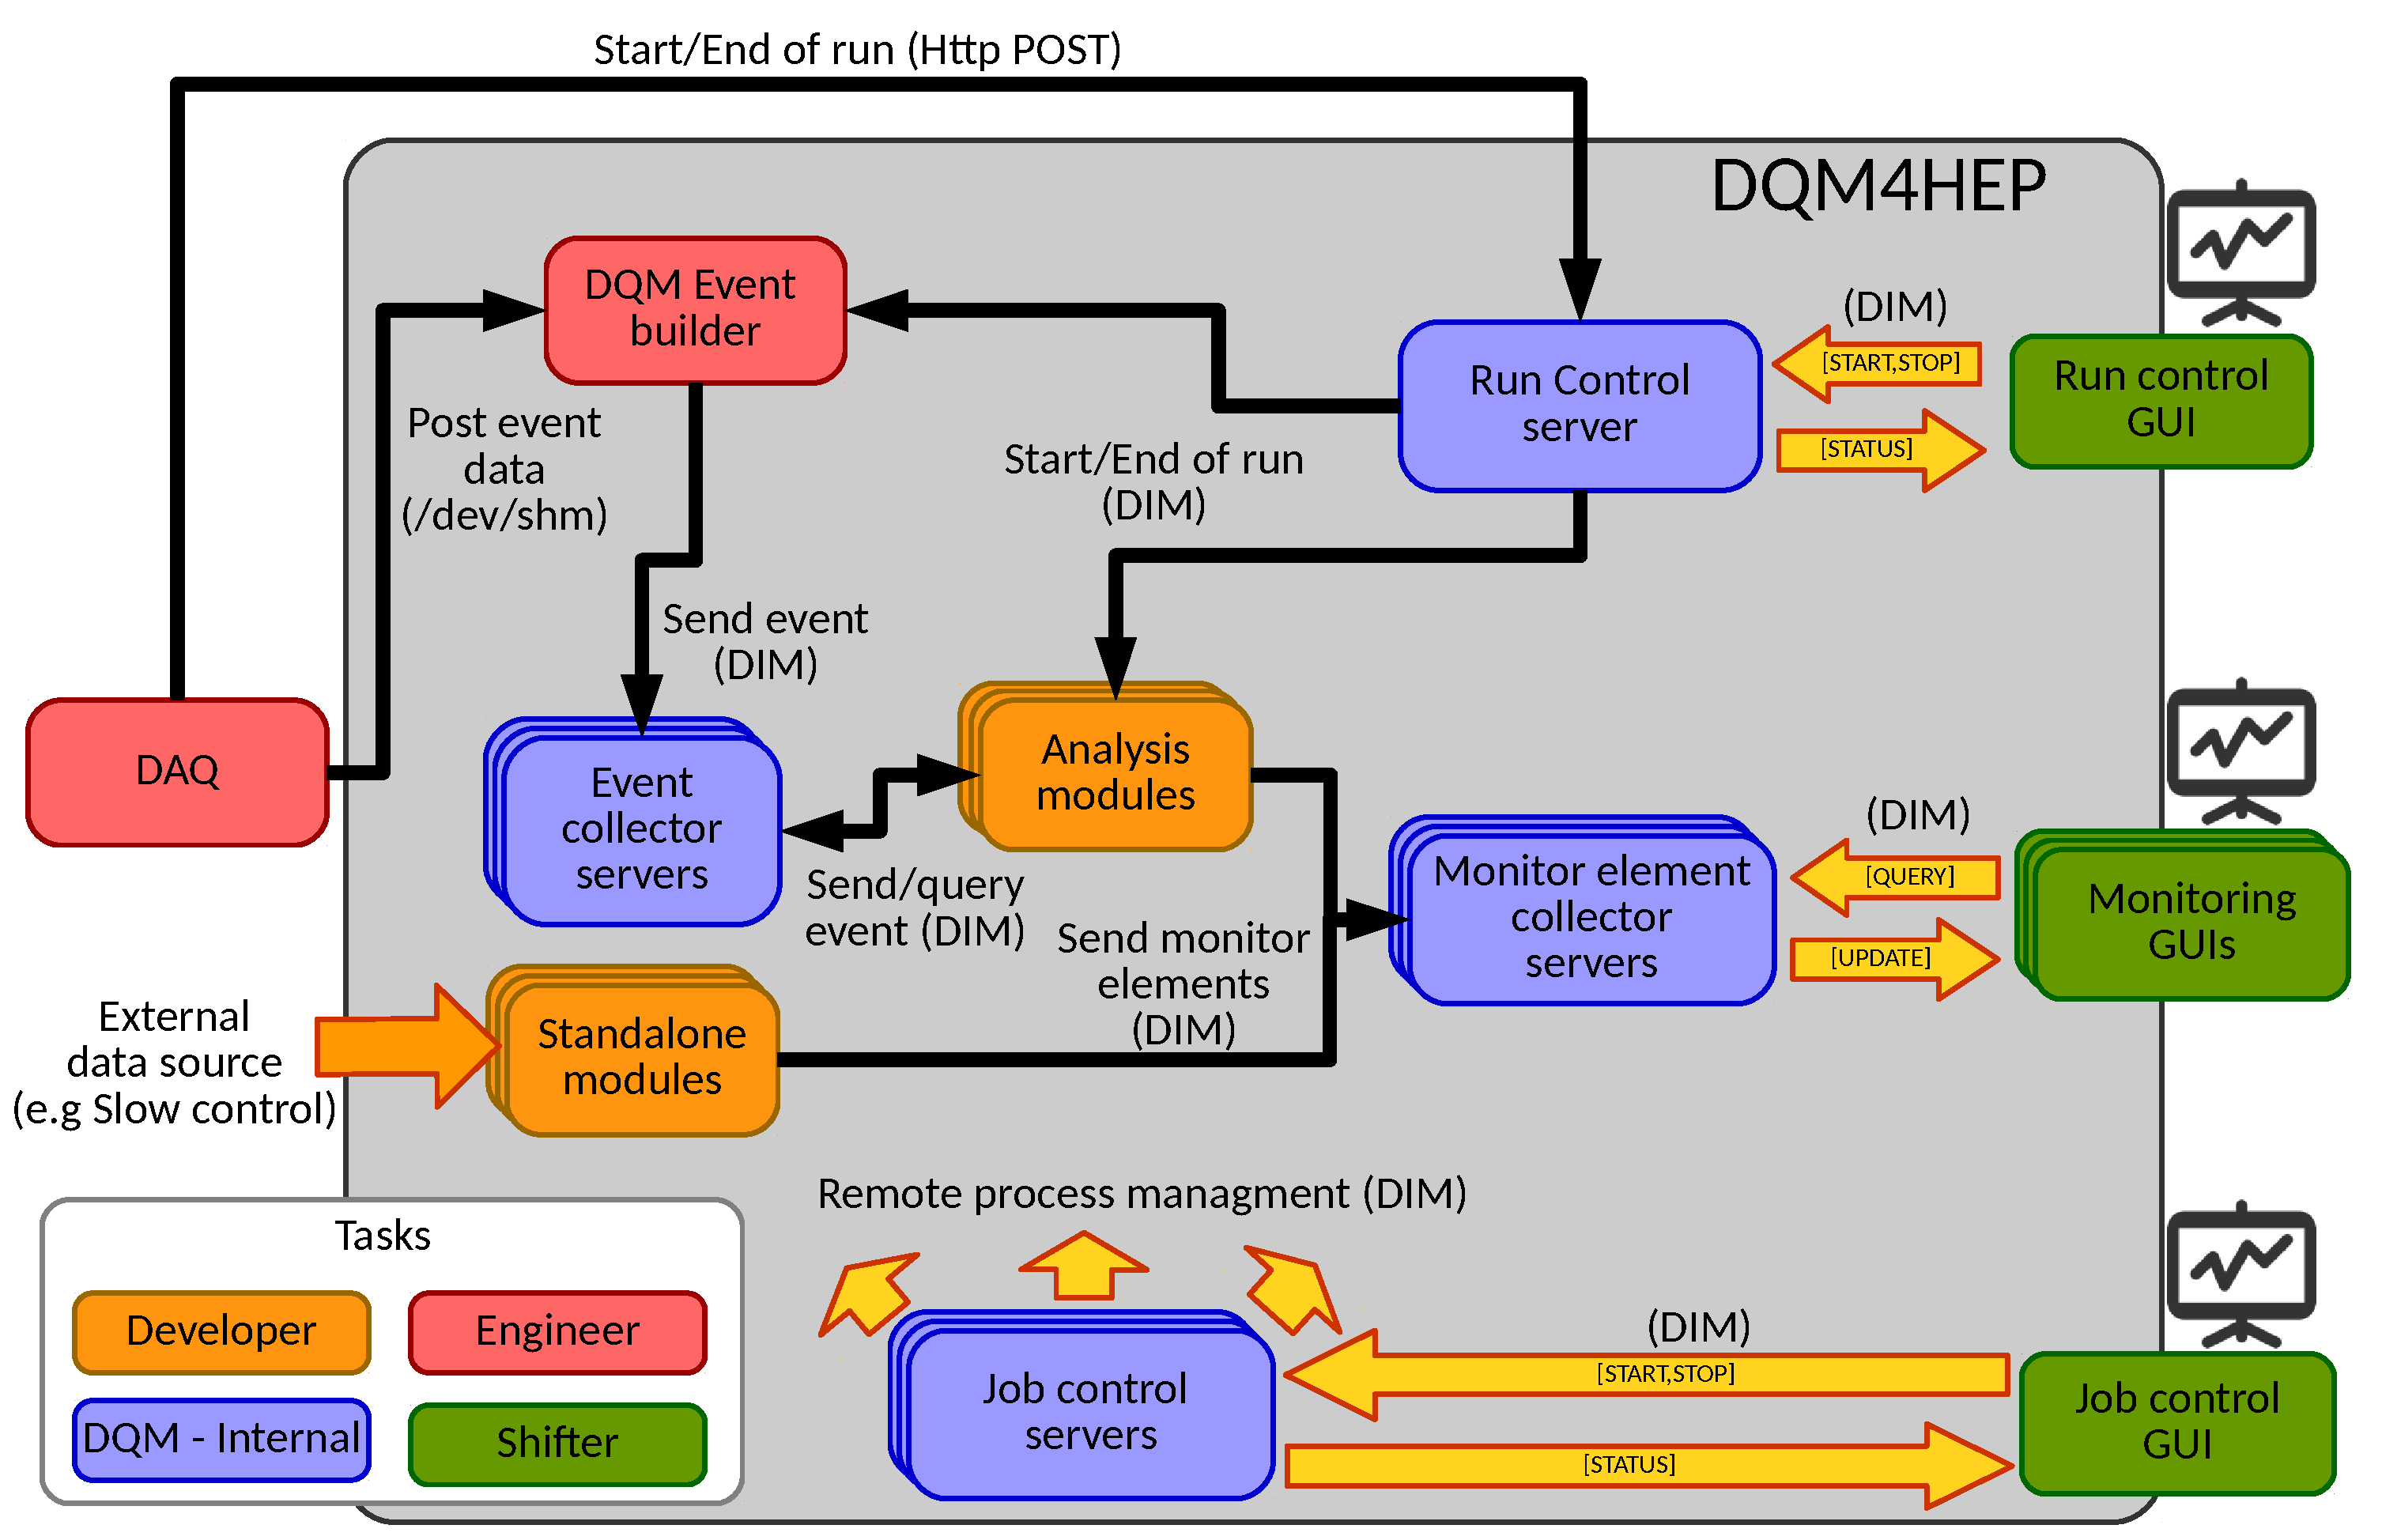
\includegraphics[width=0.9\linewidth]{figs/GlobalArchitectureDiagram.pdf}
\end{frame}

%----------------------------------------------------------------------
\begin{frame}
  \frametitle{DQM4HEP}
  \framesubtitle{Online data analysis module}
  \scriptsize
  \begin{block}{Analysis module}
    \begin{itemize}
      \item \textbf{Receive and process event (e.g from DAQ)}
      \item Book and fill histograms
      \item Process quality tests
      \item Send histogram and QReports to collectors with cycle structure
      \begin{itemize}
        \scriptsize
        \item Every N events/seconds
        \item User can reset histogram if needed at end of cycle
      \end{itemize}
    \end{itemize}
  \end{block}
  \begin{block}{Standalone module}
    \begin{itemize}
      \item \textbf{Receive and process data from external source (e.g slow control)}
      \item Book and fill histograms
      \item Process quality tests
      \item Send histogram and QReports to collectors every N seconds
    \end{itemize}
  \end{block}
\end{frame}

%----------------------------------------------------------------------
% \begin{frame}
%   \frametitle{DQM4HEP}
%   \framesubtitle{Slow control module}
%   \centering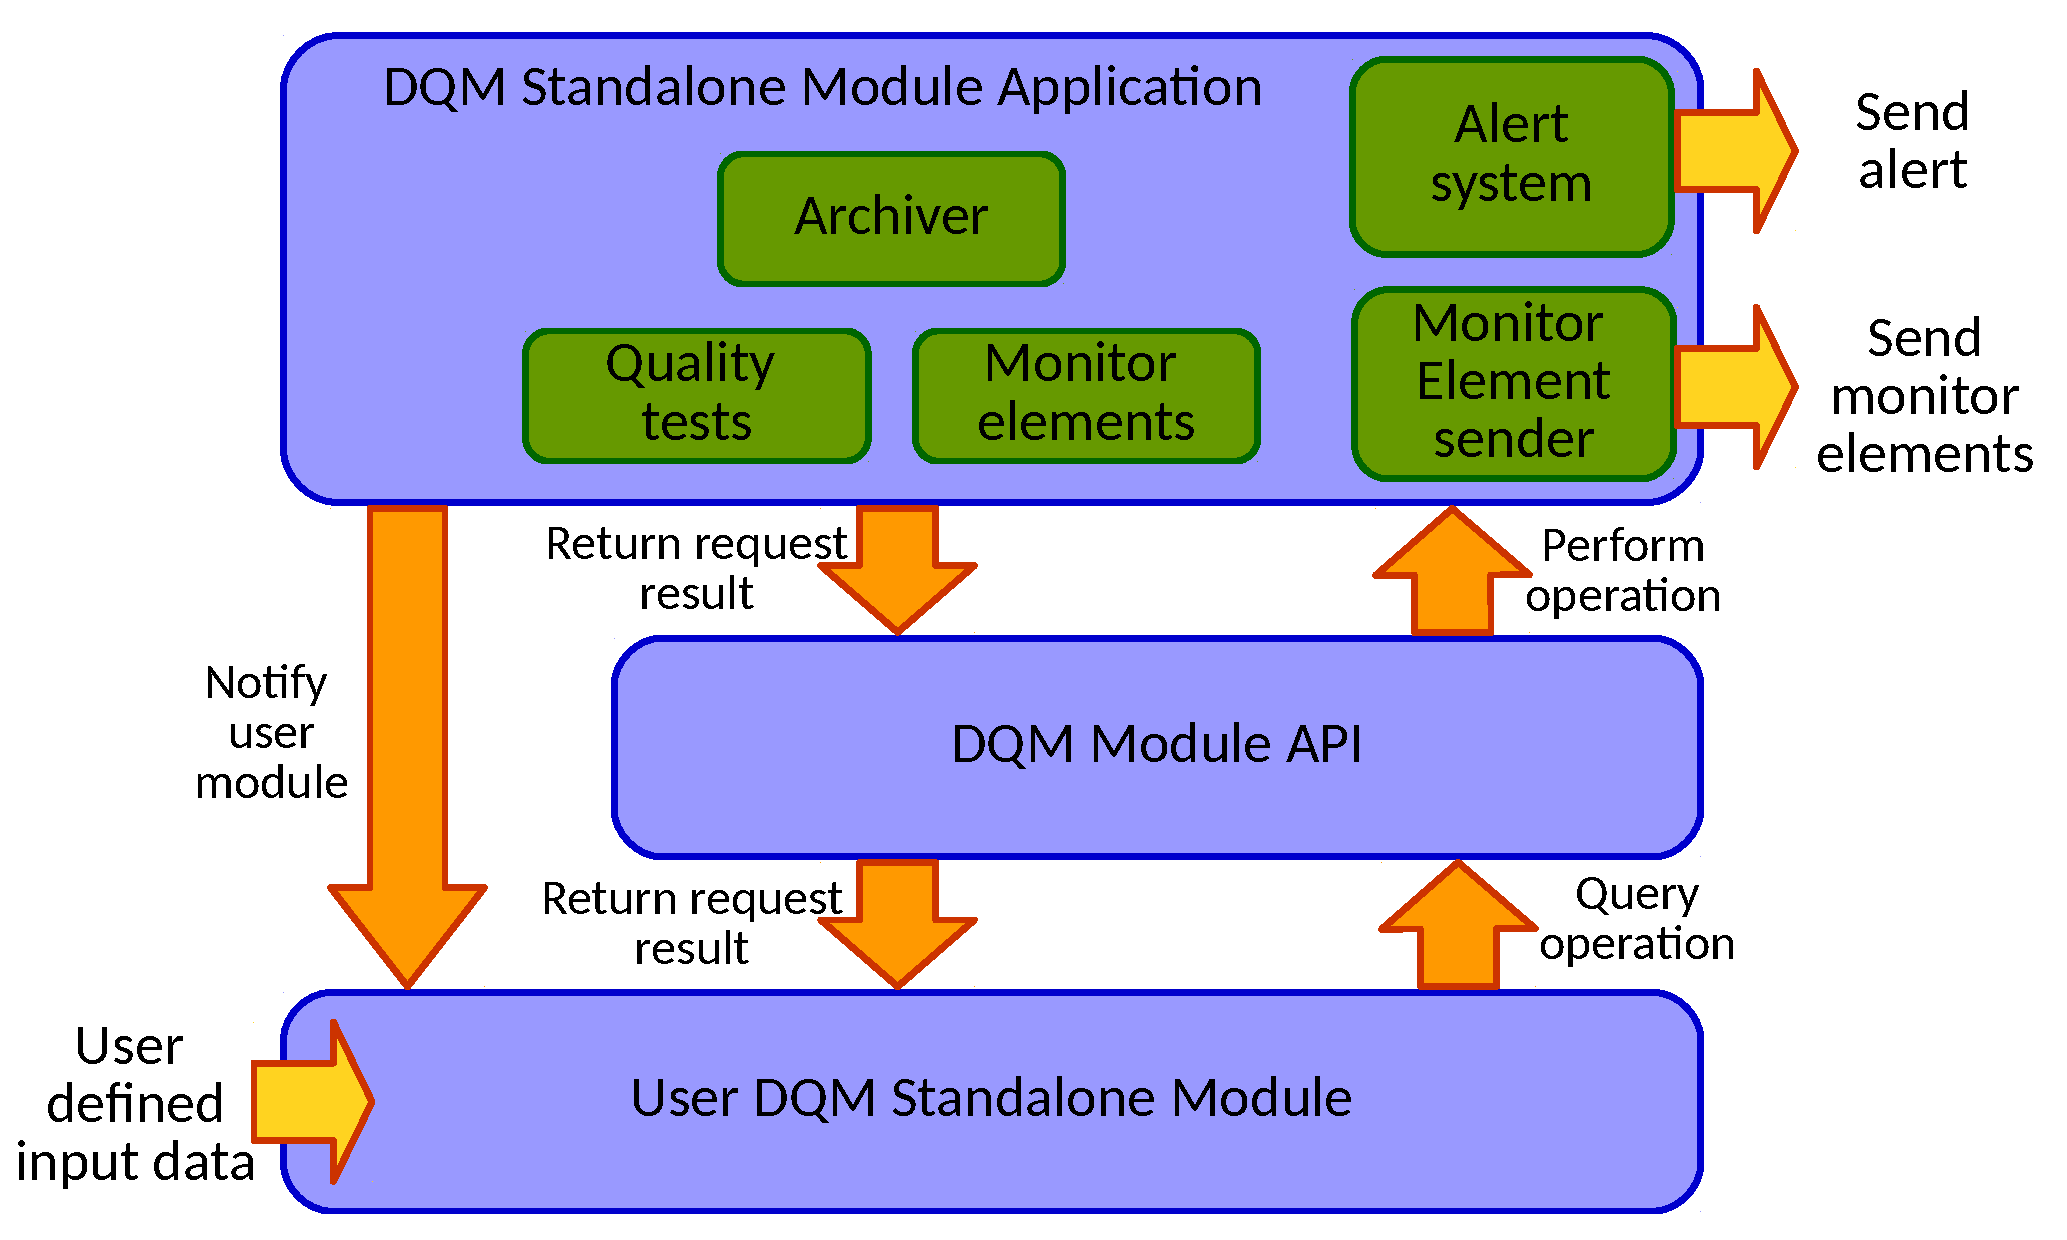
\includegraphics[width=0.9\linewidth]{figs/StandaloneModuleApplicationDiagram.pdf}
% \end{frame}

% %----------------------------------------------------------------------
% \begin{frame}
%   \frametitle{DQM4HEP}
%   \framesubtitle{Job control interface (Qt Gui)}
%     \centering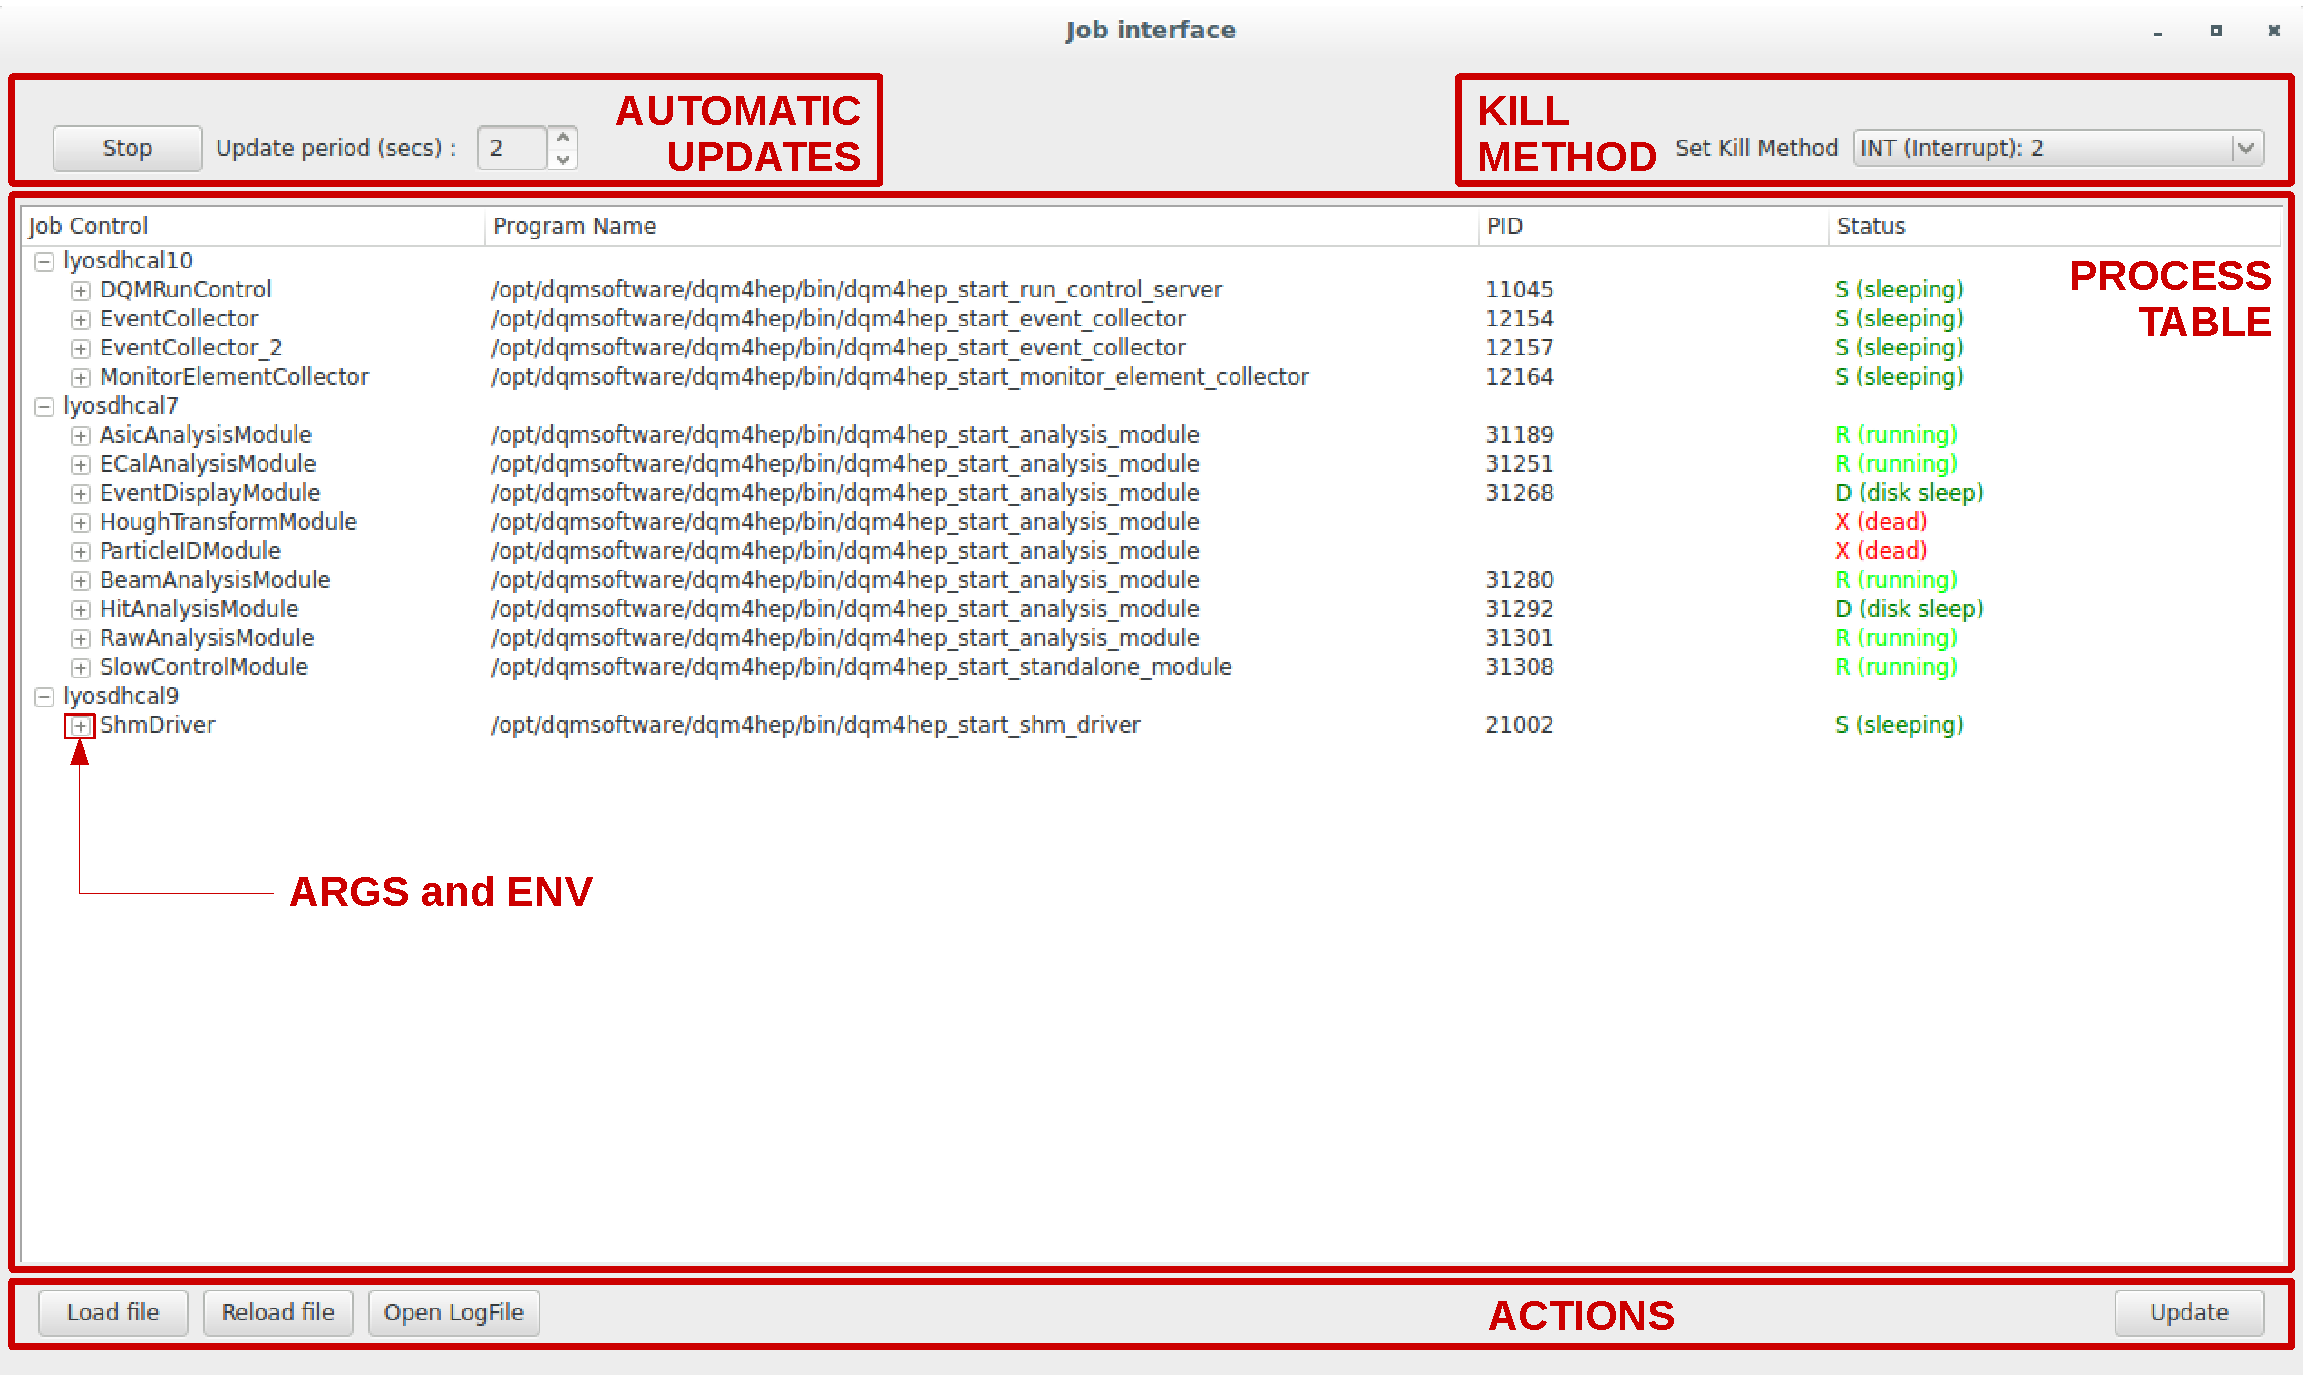
\includegraphics[width=0.95\linewidth]{figs/JobControlGui.pdf} \\
%     Start/stop/manage many processes on many hosts
% \end{frame}

% %----------------------------------------------------------------------
% \begin{frame}
%   \frametitle{DQM4HEP}
%   \framesubtitle{Online monitoring interface (Qt Gui)}
%     \scriptsize
%     \begin{center}
%       \includegraphics<1->[height=0.7\textheight]{figs/DQM4HEPMonitoringGui.png}
%       \llap{\includegraphics<2>[height=0.7\textheight]{figs/Browser_Search.pdf}}
%     \end{center}
%     \vspace{-0.7cm}
%     \begin{minipage}{0.49\linewidth}
%       \begin{itemize}
%         \item Histograms organized in tree structure
%         \item Plot many histograms at the same time
%       \end{itemize}
%     \end{minipage}
%     \begin{minipage}{0.49\linewidth}
%       \begin{itemize}
%         \item Receive real time updates
%         \item Browse histograms on collectors
%       \end{itemize}
%     \end{minipage}
% \end{frame}

% %----------------------------------------------------------------------
% \begin{frame}
%   \frametitle{DQM4HEP}
%   \framesubtitle{Detectors using DQM4HEP}
%   \footnotesize
%   DQM4HEP used by different detectors in the CALICE collaboration. \\
%   \scriptsize
%   ~\\
%   \begin{minipage}{0.4\linewidth}
%     SDHCal online monitoring
%     \begin{itemize}
%       \item Hit maps
%       \item Electronics rate
%       \item Slow control : I, HV, LW, T, P
%       \item GRPC efficiency, multiplicity
%     \end{itemize}
%     ~\\
%     ~\\
%     ~\\
%     ~\\
%     ~\\
%     AHCal online monitoring
%     \begin{itemize}
%       \item Hit maps
%       \item Correlation with Telescope hits
%       \item Electronics rate
%     \end{itemize}
%   \end{minipage}
%   \begin{minipage}{0.59\linewidth}
%     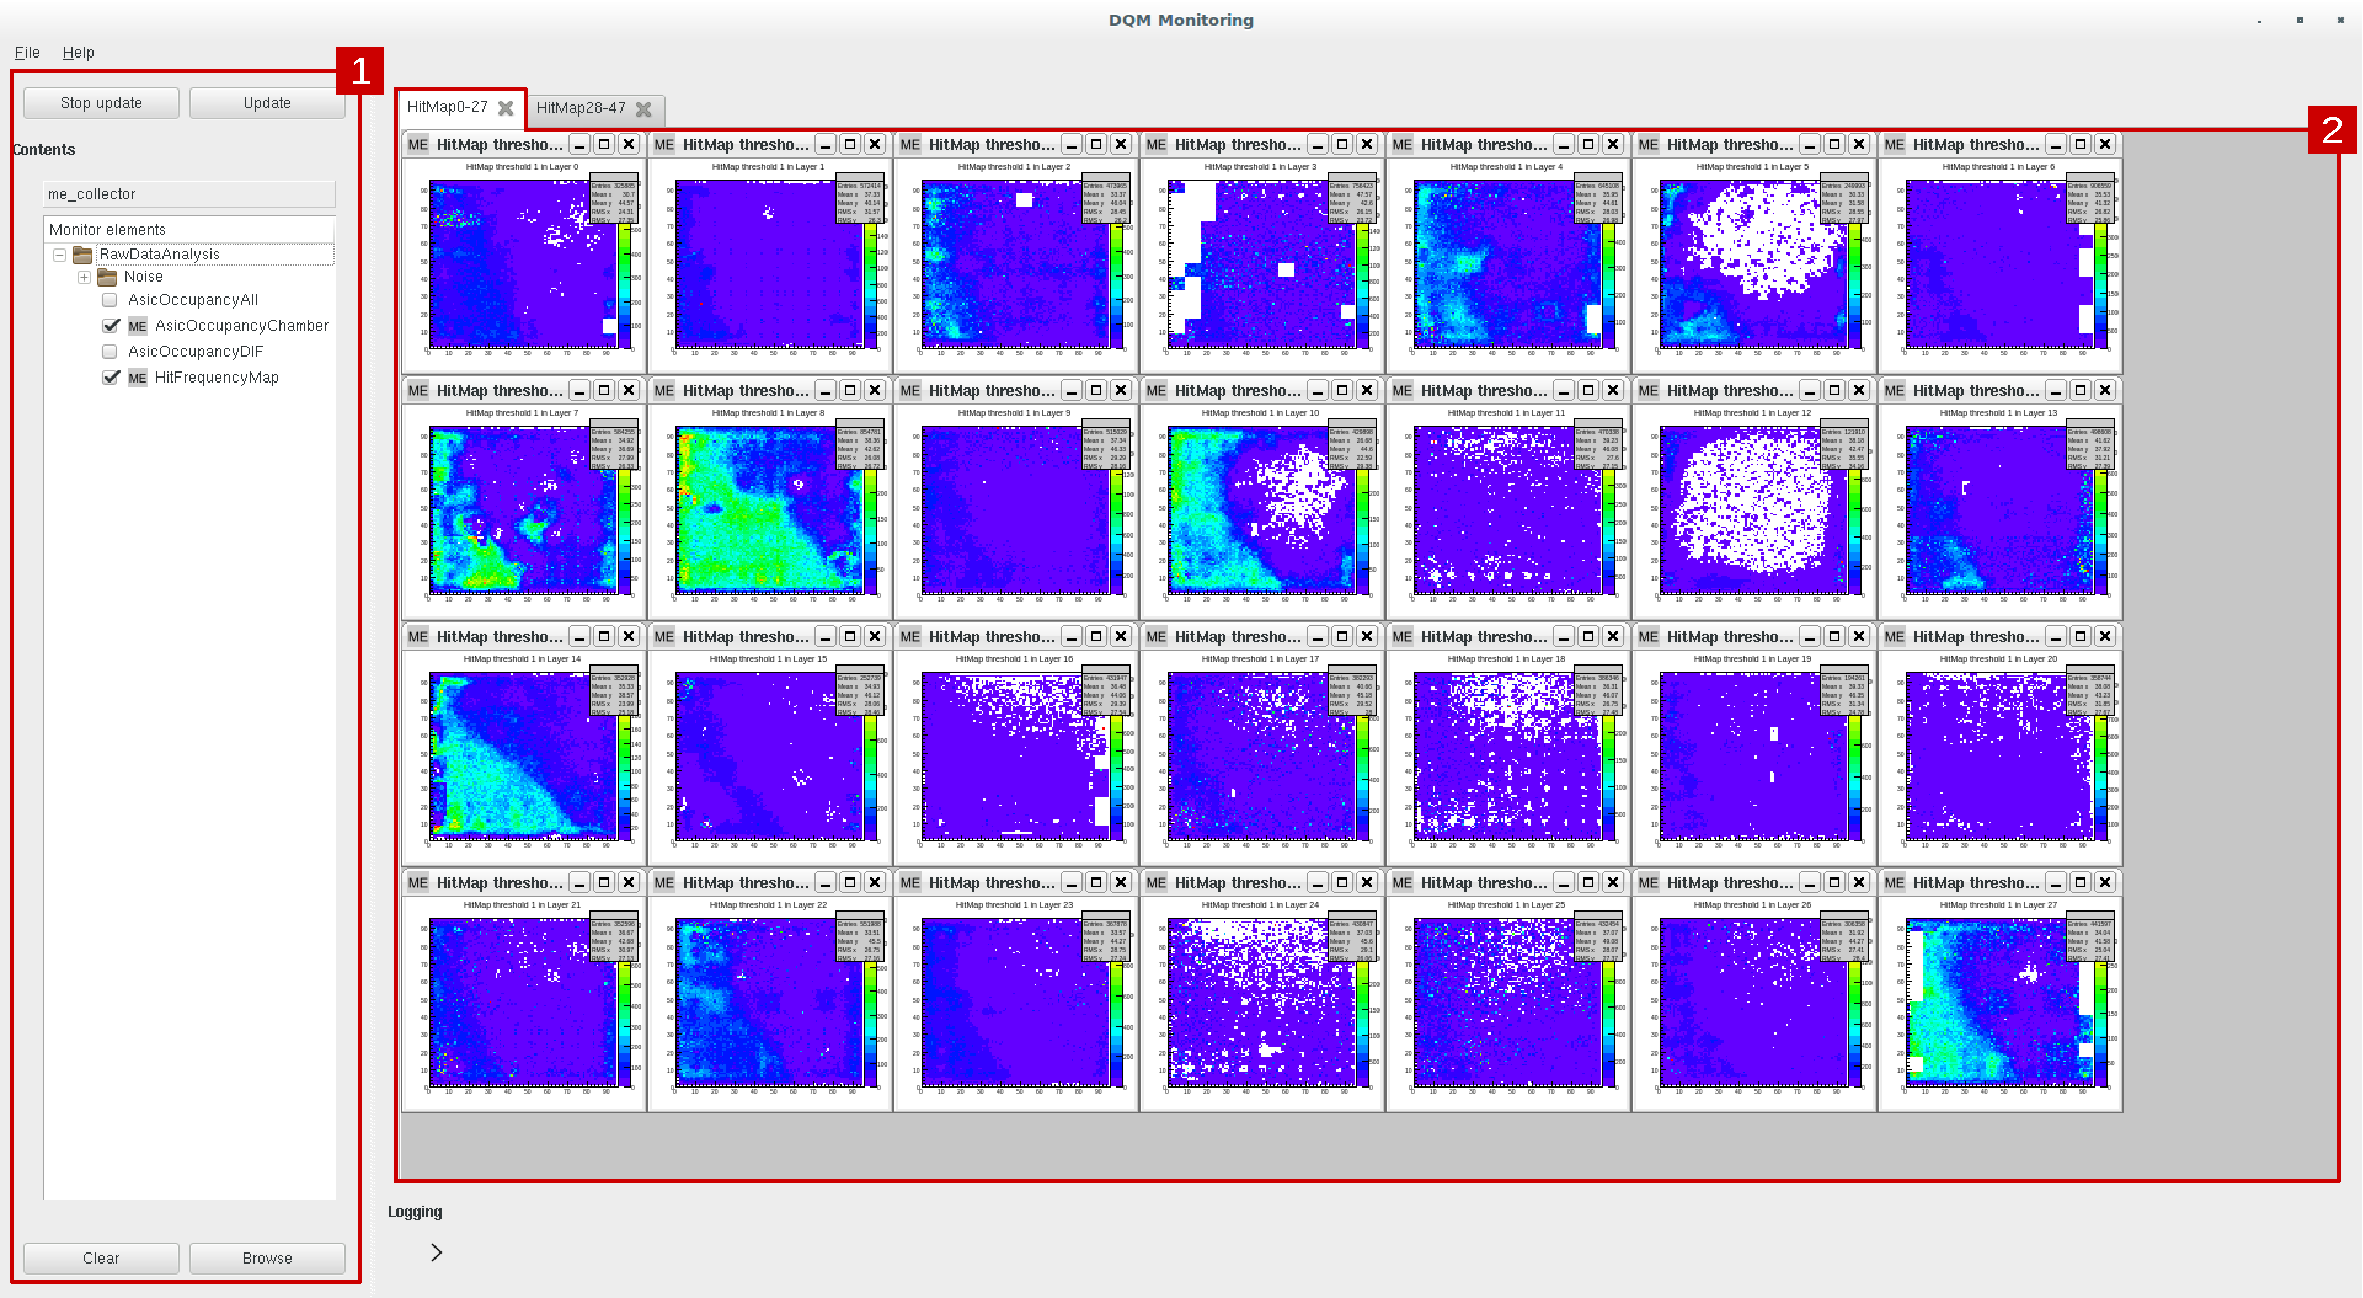
\includegraphics[width=0.95\linewidth]{figs/MonitoringMainWindowGui.pdf} \\
%     ~\\
%     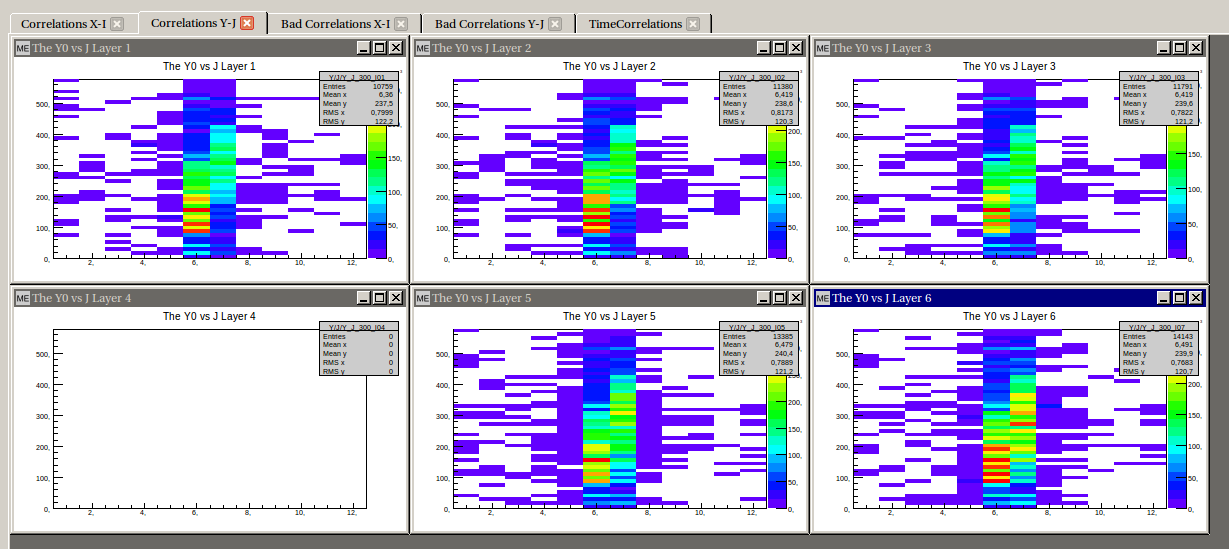
\includegraphics[width=0.95\linewidth]{figs/AHCal_DQM4HEP_CorrelationsYJ.png}
%   \end{minipage}
% \end{frame}

%----------------------------------------------------------------------
\begin{frame}
  \frametitle{DQM4HEP}
  \framesubtitle{EUDAQ binding}
  \scriptsize
  Binding between the EUDAQ framework and DQM4HEP is ongoing.\\
  ~ \\
  Need to :
  \begin{itemize}
    \item implement event streamer plugin
    \item implement the run control interface
    \item integrate DQM4HEP in EUDAQ
  \end{itemize}
  ~ \\
  Possible EUDAQ update to use DQM4HEP : \\
  ~ \\
  \begin{minipage}{0.49\linewidth}
    \centering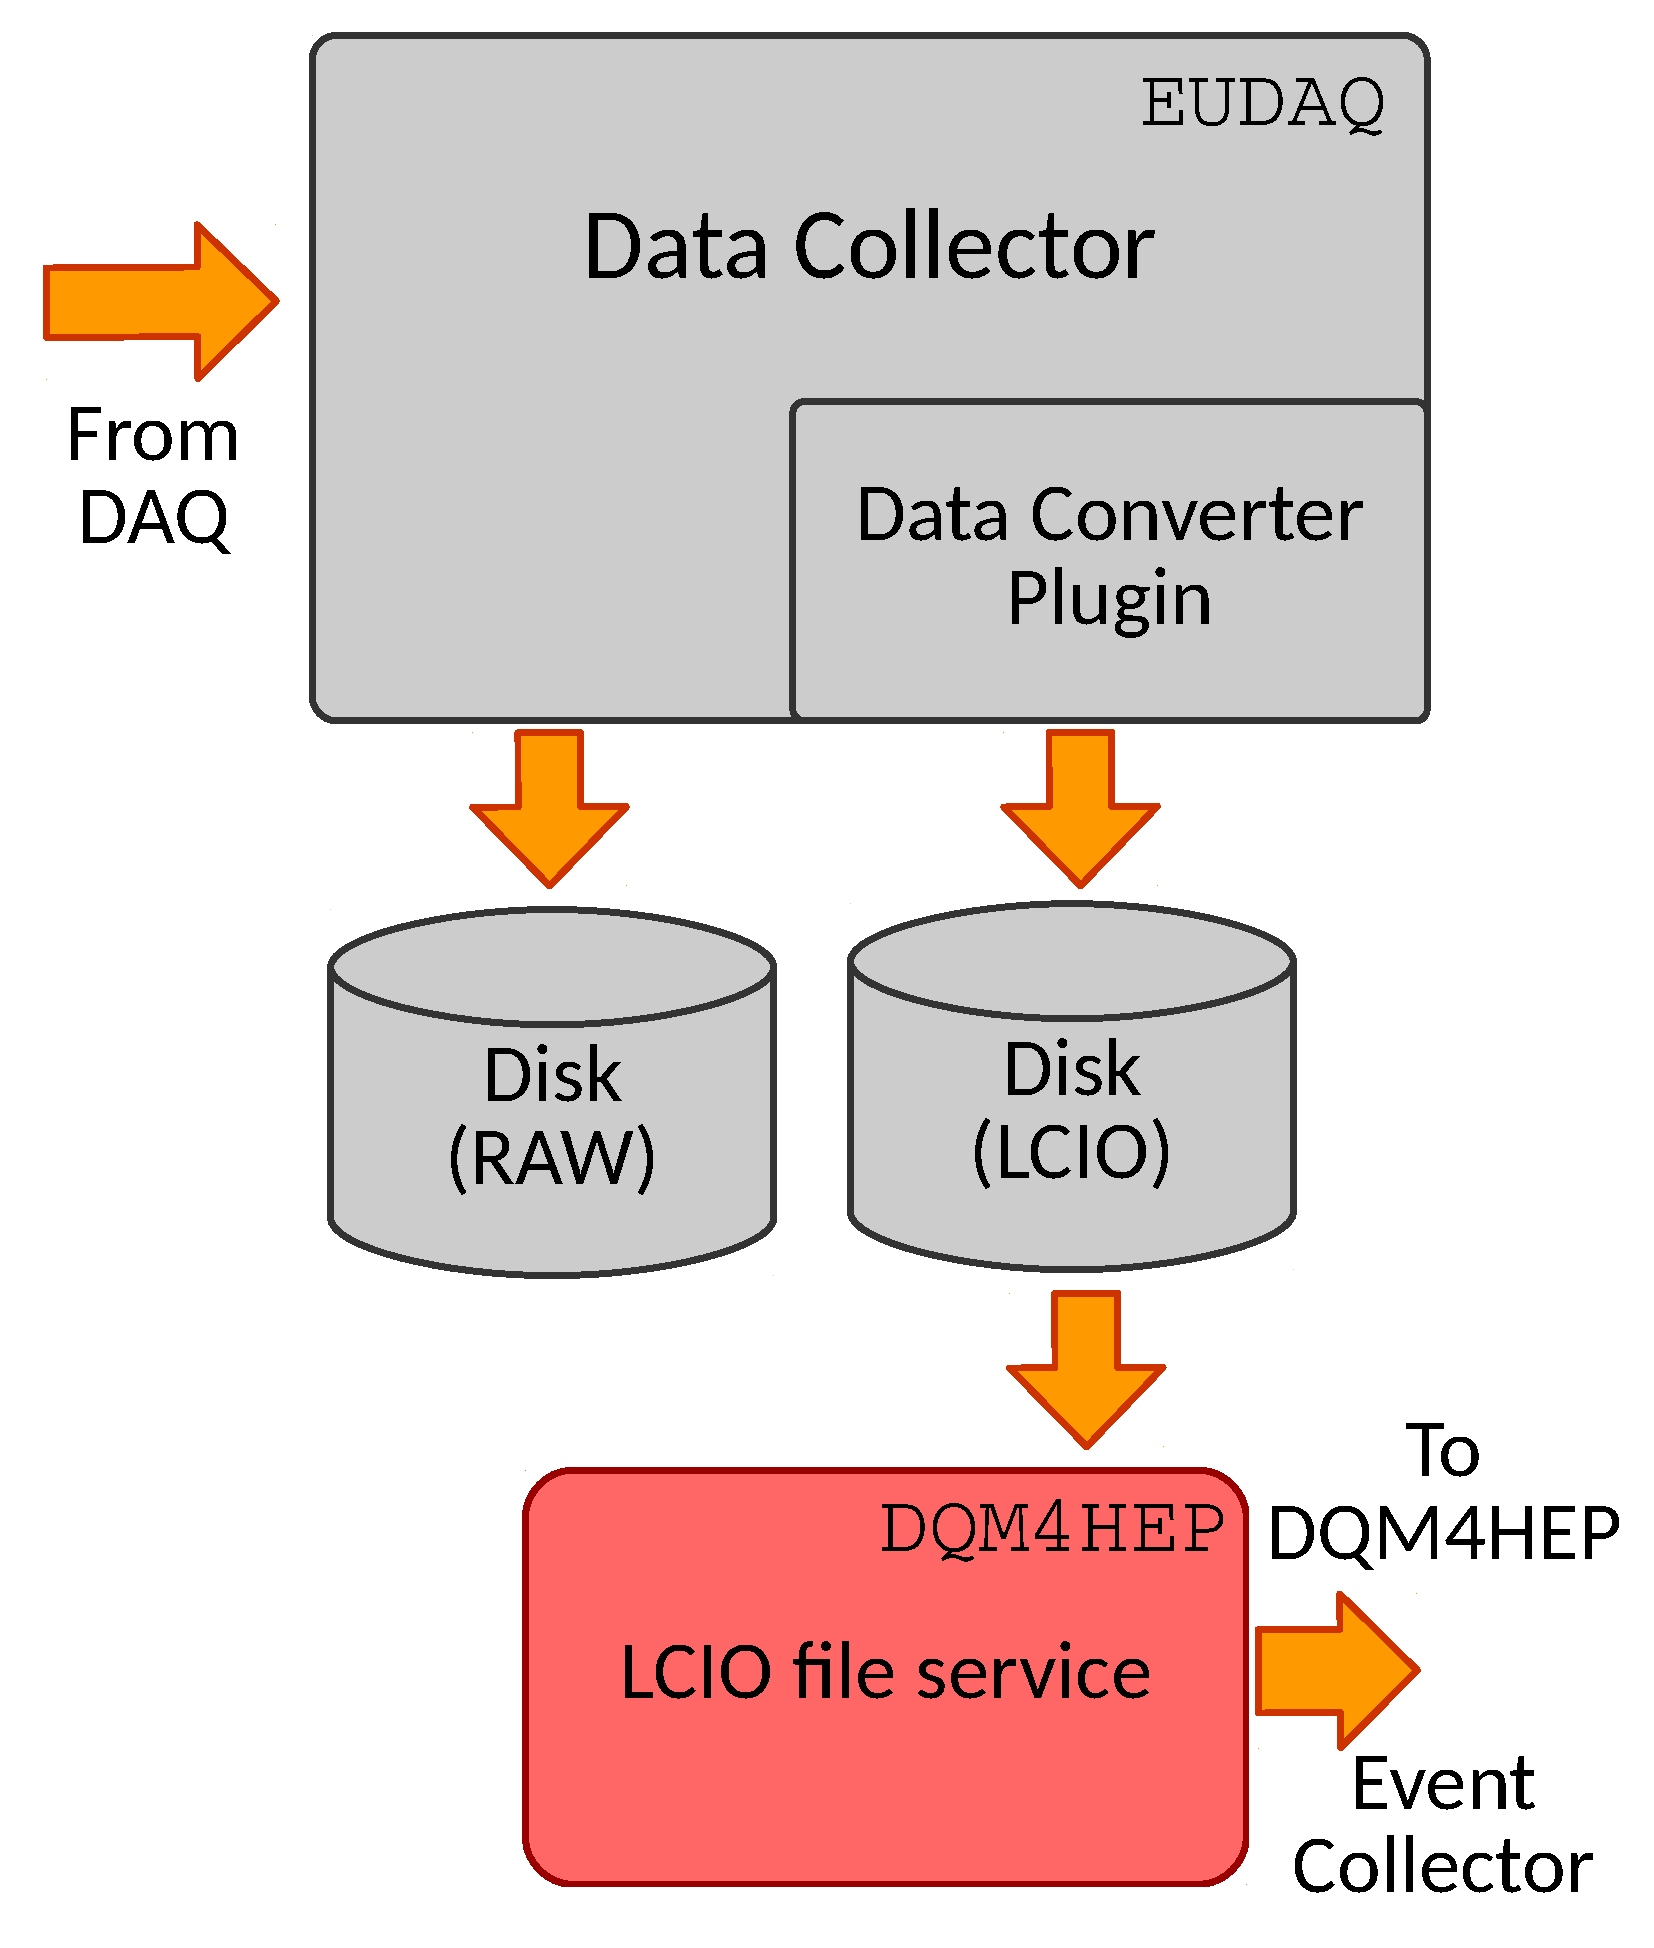
\includegraphics[width=0.6\linewidth]{figs/EUDAQ-DQM4HEP-Current.pdf}
  \end{minipage}
  \begin{minipage}{0.49\linewidth}
    \centering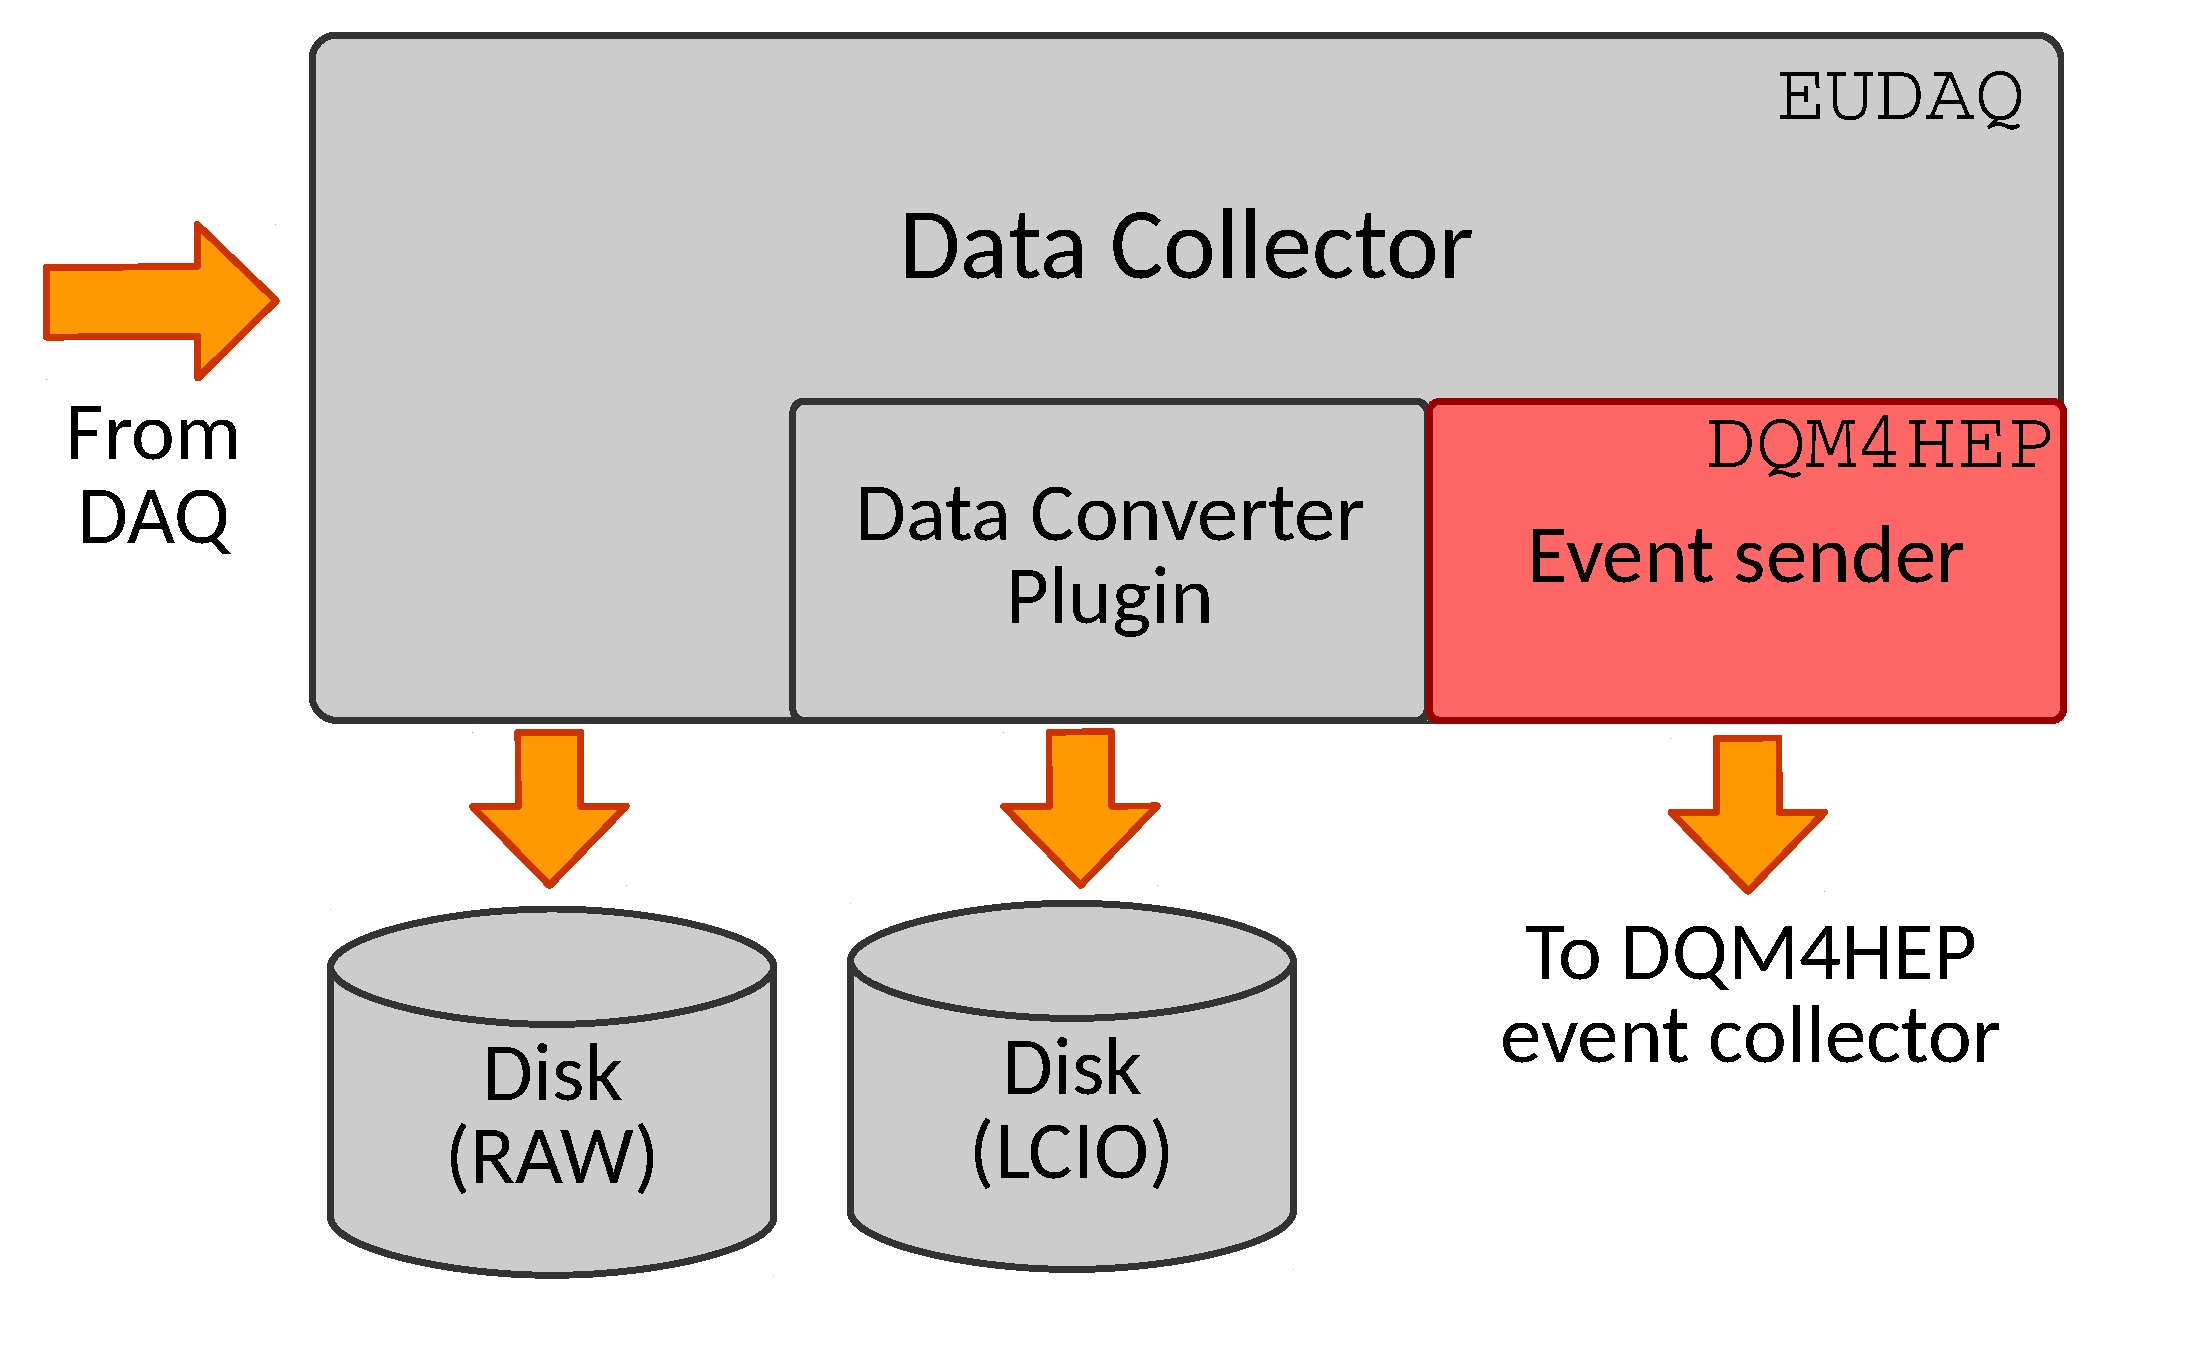
\includegraphics[width=0.8\linewidth]{figs/EUDAQ-DQM4HEP-Ongoing.pdf}
  \end{minipage} \\
  ~ \\
  \begin{minipage}{0.49\linewidth}
    \centering Current
  \end{minipage}
  \begin{minipage}{0.49\linewidth}
    \centering Foreseen
  \end{minipage}
\end{frame}

%----------------------------------------------------------------------
\begin{frame}
  \frametitle{DQM4HEP}
  \framesubtitle{Ongoing work on framework}
  \footnotesize
  ILD collaboration entering in a new MC production process. \\
  ~ \\
  Need for automatic data quality checks for simulated/reconstructed quantities. \\
  ~ \\
  Ongoing work to separate the main package (DQMCore) into two different software \\
  ~\\
  \begin{minipage}{0.49\linewidth}
    \textbf{dqm4hep-core}
  \end{minipage}
  \begin{minipage}{0.49\linewidth}
    \textbf{dqm4hep-online}
  \end{minipage} \\
  ~ \\
  \begin{minipage}{0.49\linewidth}
    \begin{itemize}
      \scriptsize
      \item MonitorElement (ROOT)
      \item Quality test
      \item Event interface
      \item Streaming (xdrstream)
      \item Plugin management
      \item DB tools (MySQL)
      \item Logging (spdlog)
    \end{itemize}
  \end{minipage}
  \begin{minipage}{0.49\linewidth}
    \begin{itemize}
      \scriptsize
      \item Modules (User classes, Online API)
      \item Event collector (server and client)
      \item Monitor element collector (server and client)
      \item Run control (server, client and external interface)
    \end{itemize}
  \end{minipage}
\end{frame}

%----------------------------------------------------------------------
\begin{frame}
  \frametitle{DQM4HEP}
  \framesubtitle{Ongoing work on framework}
  \scriptsize
  Current effort to provide an important set of quality test templates in core library \\
  ~ \\
  Users can also implement their own quality tests \\
  ~\\
  ~\\
  \begin{minipage}{0.45\linewidth}
    \begin{itemize}
      \item \textbf{Kolmogorov test (hist + ref)}
      \item Mean withing range
      \item Mean 90 within range
      \item No data after limit
      \item No data before limit
      \item \textbf{Fit function and check $\chi^2$}
      \item Likelihood fit
      \item Fraction of data after limit exceed
      \item Fraction of data before limit exceed
      \item RMS lower than
      \item RMS 90 lower than
    \end{itemize}
  \end{minipage}
  \begin{minipage}{0.53\linewidth}
    \begin{itemize}
      \item RMS greater than
      \item RMS 90 greater than
      \item Mean lower than
      \item Mean 90 lower than
      \item Mean greater than
      \item Mean 90 greater than
      \item RMS within range
      \item RMS 90 within range
      \item \textbf{Fit function and check parameters within range}
      \item Distance between two values
    \end{itemize}
  \end{minipage} \\
  ~\\
  ~\\
  Incoming work : \textbf{possibility to test any object in ROOT files using these quality tests}
\end{frame}


%----------------------------------------------------------------------
\begin{frame}
  \frametitle{DQM4HEP}
  \framesubtitle{Timeline}
  \footnotesize
  Current work \\
  \begin{itemize}
    \item Quality tests (Tom) : 2 months
    \item Core tools (Remi) : 2 months
  \end{itemize}
  ~ \\
  Future work \\
  \begin{itemize}
    \item Online package under total review
    \begin{itemize}
      \scriptsize
      \item Online architecture remains the same
      \item Change networking layer (dqm4hep-net)
    \end{itemize}
    \item Implement EUDAQ$\leftrightarrow$DQM4HEP interface
    \item Develop web interface to replace
    \begin{itemize}
      \scriptsize
      \item Monitoring GUI
      \item Job control
      \item Framework status
    \end{itemize}
  \end{itemize}
\end{frame}

%----------------------------------------------------------------------
% \begin{frame}
%   \frametitle{DQM4HEP}
%   \framesubtitle{Conclusion}
%   \small
%   Conclusion \\
%   \begin{itemize}
%     \item Development of a new \textbf{generic framework} for data quality monitoring
%     \item Used during test-beam by different detectors and \textbf{combination of sub-detectors}
%     \item Current implementation works for online setup
%   \end{itemize}
%   ~ \\
%   Perspectives \\
%   \begin{itemize}
%     \item Refactoring of the framework to make it working for \textbf{offline data quality monitoring}
%     \item Development of a EUDAQ binding for online data taking
%     \item Development of quality test templates
%   \end{itemize}
%
% \end{frame}


%----------------------------------------------------------------------
\begin{frame}
  \frametitle{DQM4HEP}
  \framesubtitle{URLs and contact}
  GitHub collaboration\\
  \vspace*{0.1cm}
  ~~~
  \begin{minipage}{0.03\linewidth}
    
\includegraphics[width=\linewidth]{figs/github-logo.png}
  \end{minipage}
  \href{https://github.com/dqm4hep}{\tt https://github.com/dqm4hep} \\
  ~\\
  Installation package (\texttt{v04-03-00}) \\
  \vspace*{0.1cm}
  ~~~
  \begin{minipage}{0.03\linewidth}
    
\includegraphics[width=\linewidth]{figs/github-logo.png}
  \end{minipage}
  \href{https://github.com/dqm4hep/dqm4hep}{\tt https://github.com/dqm4hep/dqm4hep} \\
  ~\\
  Slack channel (Announcements, issues, management) \\
  \vspace*{0.1cm}
  ~~~
  \begin{minipage}{0.035\linewidth}
    
\includegraphics[width=\linewidth]{figs/slack-logo.png}
  \end{minipage}
  \href{https://dqm4hep.slack.com}{\tt https://dqm4hep.slack.com} \\
  ~\\
  Contact us !
  \begin{itemize}
    \item R. Ete (\href{mailto:remi.ete@desy.de}{\tt remi.ete@desy.de})
    \item A. Pingault (\href{mailto:antoine.pingault@ugent.be}{\tt antoine.pingault@ugent.be})
    \item T. Coates (\href{mailto:tc297@sussex.ac.uk}{\tt tc297@sussex.ac.uk})
  \end{itemize}
\end{frame}

\end{document}

% Enable spell checker for vim
% setlocal spell spelllang=en
